% -------------------------------------------------------------------------
% PREAMBLE: Don't modify this section unless you know what you're doing!
% -------------------------------------------------------------------------

\documentclass[letterpaper,12pt]{article}
\renewcommand{\baselinestretch}{1.3} % 1.3 linespacing
% \usepackage{indentfirst}
\usepackage{tabularx} % extra features for tabular environment
\usepackage{amsmath}  % improve math presentation
\usepackage{siunitx}  % improve math spacing
\usepackage{graphicx} % takes care of graphics inclusion machinery
\graphicspath{{./images/}}

\usepackage[margin=1in,letterpaper]{geometry} % decreases margins
% \usepackage{cite} % takes care of citations
\usepackage{caption}
\usepackage{natbib}
\usepackage[final]{hyperref} % adds hyper links inside generated PDF files
\hypersetup{
    colorlinks=true,       % false: boxed links; true: colored links
    linkcolor=blue,        % color of internal links
    citecolor=blue,        % color of links to bibliography
    filecolor=magenta,     % color of file links
}
\captionsetup[table]{
    format=hang,
    labelfont=bf,
    textfont=normalfont,
    singlelinecheck=on,
    margin=0.5in,
}
 
\captionsetup[figure]{
    format=hang,
    labelfont=bf,
    textfont=normalfont,
    singlelinecheck=on,
    margin=0.5in,
}

%--------------------------------------------------------------------------
% end of preamble
%--------------------------------------------------------------------------

\begin{document}

%--------------------------------------------------------------------------
% Title Section
%--------------------------------------------------------------------------
\title{
\begin{center}
\hspace{-1.0em}
\includegraphics[scale=0.5]{images/cls-logo-2.png}
\end{center} 
Weekly Report: May 6-12, 2019
\author{Michael Bree}
\date{\today}}
\maketitle

%--------------------------------------------------------------------------

\section{Accomplishments This Week}

In this section list accomplishments for the week. It is really easy to itemize points. For example:
\begin{itemize}
    \item This is a bullet point.
    \item Another Item
    \item \textbf{Bold} text can be used, so can \textit{italics} or even \textbf{\textit{both}}.
\end{itemize}
If one prefers, numbered items can be used.  For example, this week, I:
\begin{enumerate}
    \item created a simple {\LaTeX} template for weekly reports,
    \item began work on my EPICS presentation (currently it is about 1/2 complete), and
    \item vowed to never use Word again.
\end{enumerate}

It is really easy to insert equations.  When they are labeled as is Eq.~(\ref{eq:test_equation}), references are automatically generated:

% --------------------------------------------------------------------------
% Example equation with label
% --------------------------------------------------------------------------

\begin{equation}\label{eq:test_equation}
W_d = \dfrac{1}{\sqrt{1 + x(d/d_{pass})^n}}
\vspace{0.2in}
\end{equation}

Figures are easily inserted.  Like equations, they can be labeled and referenced.  For example, see Fig.~\ref{fig:butterworth_wait}.  If you are looking at the source for this document, the tilde (\~{})
between the Fig. and the reference suppresses line breaks there.  The nice thing about {\LaTeX}  
is that it automatically places things like Figures so you don't have to.

% --------------------------------------------------------------------------
% Example Figure
% --------------------------------------------------------------------------

\begin{figure}[ht] 
\centering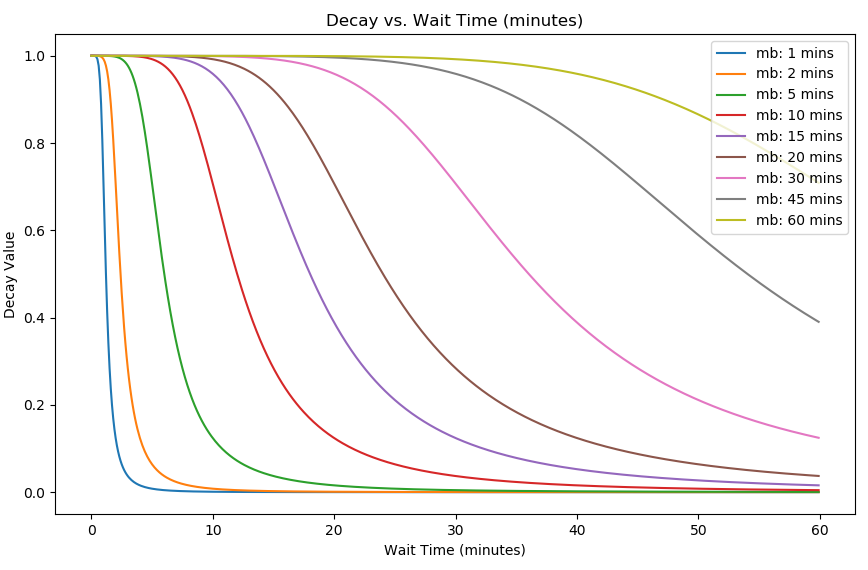
\includegraphics[width=1.0\columnwidth]{butterworth_wait}
\caption{Decay (e.g., in attitude) vs. Wait Time (e.g., for cable guy) for various values of $mb$ (e.g., meaningful benefit). \label{fig:butterworth_wait}}
\end{figure}

References are easy to manage, and in fact Overleaf supports integration with \textit{Zotero}, a popular reference manager. Using Zotero, you do not have to manually format references like this one:~\cite{knuth:1984}. It is very easy to change the reference style, and the References section itself is completely auto-generated. 

A snippet of source code can be shown as follows:

\linespread{1}\begin{verbatim}
    import sys
    import os
    print "Hello World"
\end{verbatim}

Tables are easy too! See example in Table~\ref{table:example_table}. Of course there is a wide range of table formats available.   The point of this sentence is to extend the text down to the footer.  The point of this sentence is to extend the text down to the footer.  The point of this sentence is to extend the text down to the footer.  The point of this sentence is to extend the text down to the footer.  

% --------------------------------------------------------------------------
% Example Table
% --------------------------------------------------------------------------

\begin{table}[ht] % "h" means try to put it here (h! means do it)
\centering\setlength{\tabcolsep}{18pt}
\begin{tabular}{cccc}
\textbf{Thing} & \textbf{Value 1} & \textbf{Value 2} & \textbf{Value 3} \\
& (description) & (description) & (description)\\
\hline
A &  3 & 3 &  3     \\
B &      & 2 & 2\\
C &      &     & 3    \\
D & 1  & 1 &        \\
E & 1  & 1 &        \\
\hline
\end{tabular}
\caption{Things, their values, and descriptions of those values.  A long table caption should wrap properly.}
\label{table:example_table}
\end{table}

\section{Goals for Next Week}

My goals for next week include:
\begin{itemize}
    \item Completing my EPICS presentation.
    \item Finishing the \textbf{\textit{Point Vortex Scan}} in PyAcq.
\end{itemize}

\bibliographystyle{agsm}
\bibliography{references.bib} 
\end{document}
